 \section{Composite Property Chain ODP}\begin{description}
\item [CLASSIFICATION:] Domain Modelling.

\item [MOTIVATION:] A composite chain can be appreciated by the following example: the son of the brother of my father is my cousin. The same structure can be applied for modelling, for example, the sucessive modifications that a protein goes through. The key on the composite chain is that there are two chains, but one of them is composed by a relationship that will be inferred by the reasoner: the reasoner will first infer that the brother of my father is my uncle (first chain: father + brother = uncle), and then that the son of my uncle is my cousin (second chain: uncle + son = cousin). The property uncle is common to both chains.

\item [AIM:] To model a double chain of properties, i.e. two chains that link four individuals.

\item [STRUCTURE:] See Figure \ref{odp:Composite_Chain_abstract}.
\begin{figure}[]\centering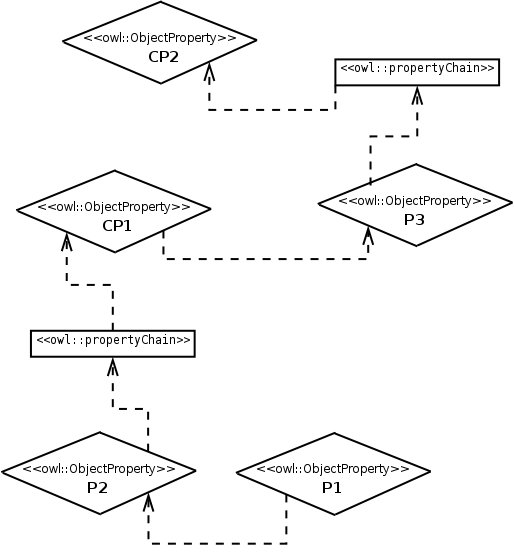
\includegraphics[width=\textwidth]{Catalogue/Composite_Chain_abstract}\caption{\label{odp:Composite_Chain_abstract} Abstract structure of the Composite Property Chain ODP.}\end{figure}

\item [SAMPLE:] See Figure \ref{odp:Composite_Chain_instance}.
\begin{figure}[]\centering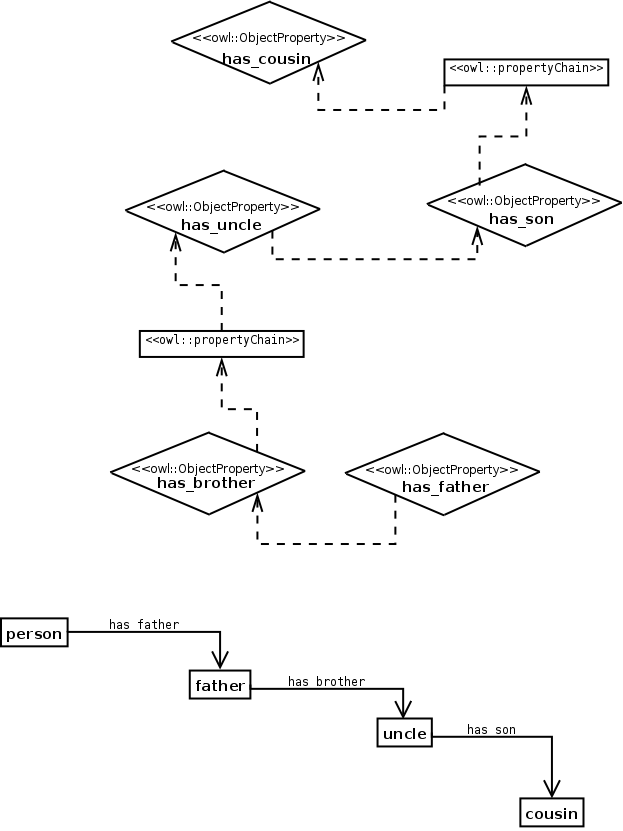
\includegraphics[width=\textwidth]{Catalogue/Composite_Chain_instance}\caption{\label{odp:Composite_Chain_instance} Sample structure of the Composite Property Chain ODP.}\end{figure}

\item [ELEMENTS:] This ODP is made by five object properties, grouped in two chains. Both chains have one object property in common: in one of them it is the head and in the other it is one of the precedents.

\item [IMPLEMENTATION:] The only main step of this ODP is to create both chains, and to link the appropriate individuals.

\item [RESULT:] The double chain is modelled. This allows for queries with the composite properties (e.g. has\_uncle and has\_cousin).

\item [REFERENCES: ] ~\begin{itemize}
\item \url{http://odps.sourceforge.net}\end{itemize}
\item [URL: ] \url{http://www.gong.manchester.ac.uk/odp/owl/Domain_Modelling_ODP/Composite_Property_Chain.owl} \end{description}